\documentclass{article}
\usepackage{amsmath}
\usepackage{amsthm}
\usepackage{amssymb}
\usepackage{enumerate}
\usepackage{graphicx}

\newenvironment{solution}{
    \par \textbf{Solution: } \quad \par
}{\par}
% done
\begin{document}
    \title{Chapter 3 Second Exercise}
    \author{Wang Yue from CS Elite Class}
    \date{\today}

    \maketitle

    \section*{Exercise 3.3}
    \subsection*{9. $y = \frac{x}{2 - \tan x}$}

    $$y' = \frac{(2 - \tan x) - x(-\sec^2 x)}{(2 - \tan x)^2}$$

    \subsection*{17. Prove that $\frac{d}{dx}(\csc x) = - \csc x \cot x$.}

    \begin{proof}
        $$(\csc x)' = (\frac{1}{\sin x})' = \frac{-\cos x}{\sin ^2 x} = -\frac{\cos x}{\sin x}\frac{1}{\sin x} = - \csc x \cot x$$

    \end{proof}

    \subsection*{18. Prove that $\frac{d}{dx}(\sec x) = \sec x \tan x$.}

    \begin{proof}
        $$(\sec x)' = (\frac{1}{\cos x})' = \frac{\sin x}{\cos ^2 x} = \sec x \tan x $$
        
    \end{proof}

    \subsection*{42. $\lim_{\theta \to 0}\frac{\cos \theta - 1}{\sin \theta}$}

    \begin{solution}
        By the equivalent infinitesimal, 
        $$\lim_{\theta \to 0}\frac{\cos \theta - 1}{\sin \theta} = \lim_{x \to 0}\frac{-\frac 1 2 x^2}{x} = 0$$
    \end{solution}

    \subsection*{44. $\lim_{x \to 0}\frac{\sin 3x \sin 5x}{x^2}$}

    \begin{solution}
        By the equivalent infinitesimal, $$\lim_{x \to 0}\frac{\sin 3x \sin 5x}{x^2} = \lim_{x \to 0}\frac{3x \times 5x}{x^2} = 15$$
    \end{solution}

    \subsection*{45. $\lim_{\theta \to 0}\frac{\sin \theta}{\theta + \tan \theta}$}

    \begin{solution}
        By the equivalent infinitesimal, $$\lim_{\theta \to 0}\frac{\sin \theta}{\theta + \tan \theta} = \lim_{x \to 0}{x}{x + x} = \frac 1 2$$
    \end{solution}

    \subsection*{47. $\lim_{x \to \frac \pi 4}\frac{1 - \tan x}{\sin x - \cos x}$}

    \begin{solution}
        $$
        \begin{aligned}
            lim_{x \to \frac \pi 4}\frac{1 - \tan x}{\sin x - \cos x} &= lim_{x \to \frac \pi 4}{1 - \frac{\sin x}{\cos x}}{\sin x - \cos x} \\
            &= \lim_{x \to \frac \pi 4}{\cos x - \sin x}{(\sin x - \cos x)\cos x} \\
            &= \lim_{x \to \frac \pi 4}{-1}{\cos x} \\
            &= -\sqrt 2
        \end{aligned}
        $$
    \end{solution}

    \subsection*{54. }

    $$|PQ| = 2 \times 10 \sin \frac{\theta}{2} = 20\sin \frac{\theta}{2}(\textrm{cm})$$

    $$A(\theta) = \frac 1 2 \pi (\frac{|PQ|}{2}) ^2 = 50\pi \sin ^2 \frac{\theta}{2}(\textrm{cm}^2)$$

    $$B(\theta) = \frac 1 2 \times 10 \times 10 \times \sin \theta = 50 \sin \theta(\textrm{cm}^2)$$

    $$\begin{aligned}
        \lim_{\theta \to 0^+}\frac{A(\theta)}{B(\theta)} &= \lim_{\theta \to 0^+}\frac{\pi \sin^2 \frac{\theta}{2}}{\sin \theta} \\
        &= \lim_{\theta \to 0^+}\frac{(1 - \cos \theta) \pi}{2\sin \theta} \\
        &= \lim_{\theta \to 0^+}\frac{\frac 1 2 \theta^2}{2 \theta} \\
        &= \lim_{\theta \to 0^+}\frac{\theta}{4} \\
        &= 0
    \end{aligned}$$

    \section*{Exercise 3.4}
    \subsection*{28. $y = \frac{e^u - e^{-u}}{e^u + e^{-u}}$}

    \begin{solution}
        $$\begin{aligned}
            y' &= \frac{(e^u + e^{-u})^2 - (e^u - e^{-u})^2}{(e^u + e^{-u})^2} \\
            &= \frac{(2e^u)(2e^{-u})}{(e^u + e^{-u})^2} \\
            &= \frac{4}{(e^u + e^{-u})^2}
        \end{aligned}$$
    \end{solution}

    \subsection{29. $F(t) = e^{t \sin 2t}$}

    \begin{solution}
        $$\begin{aligned}
            F'(t) &= e^{t \sin 2t}(\sin 2t + t \times 2\cos 2t) \\
            &= e^{t \sin 2t}(\sin 2t + 2t \cos 2t)
        \end{aligned}$$
    \end{solution}

    \subsection*{42. $y = \sqrt{x + \sqrt{x + \sqrt x}}$}

    \begin{solution}
        $$\begin{aligned}
            y' &= \frac{1}{2 \sqrt{x + \sqrt{x + \sqrt x}}}(x + \sqrt{x + \sqrt x})' \\
            &= \frac{1}{2 \sqrt{x + \sqrt{x + \sqrt x}}}(1 + \frac{1}{2 \sqrt{x + \sqrt x}}(1 + \frac{1}{2 \sqrt x})) \\
        \end{aligned}$$
    \end{solution}

    \subsection*{46. $y = [x + (x + \sin ^2 x)^3]^4$}

    \begin{solution}
        $$\begin{aligned}
            y' &= 4[x + (x + \sin^2 x)^3]^3[x + (x + \sin^2 x)^3]' \\
            &= 4[x + (x + \sin^2 x)^3]^3[1 + 3(x + \sin^2 x)^2(1 + 2\sin x \cos x)] \\
        \end{aligned}$$
    \end{solution}

    \subsection*{49. $y = e^{ax}\sin \beta x$}

    \begin{solution}
        $$\begin{aligned}
            y' &= (ae^{ax})\sin \beta x + e^{ax} \beta \cos \beta x \\
            &= e^{ax}(a \sin \beta x + \beta \cos \beta x)
        \end{aligned}$$
    \end{solution}

    \subsection*{91. Use the Chain Rule to prove the following.}

    \begin{enumerate}[(a)]
        \item The derivative of an even function is an odd funciton.
        \begin{solution}
            Let $f(x)$ is an even function, which means $f(-x) = f(x)$

            $$-f'(-x) = f'(x) \iff f'(-x) = -f'(x)$$

            So $f'(x)$ is an odd function.
        \end{solution}
        \item The derivative of an odd function is an even function.

        \begin{solution}
            Let $f(x)$ is an odd function, which means $f(-x) = -f(x)$

            $$-f'(-x) = -f'(x) \iff f'(-x) = f'(x)$$

            So $f'(x)$ is an even function.
        \end{solution}
    \end{enumerate}

    \subsection*{92. Use the Chain Rule and the Product Rule to give an alternative proof of the Quotient Rule.}

    \begin{proof}
        $$\begin{aligned}
            (\frac{f(x)}{g(x)})' &= (f(x)g(x)^{-1})' \\
            &= f'(x)g(x)^{-1} + f(x)(-g(x)^{-2}g'(x)) \\
            &= \frac{f'(x)g(x) - f(x)g'(x)}{g(x)^{2}}
        \end{aligned}$$
    \end{proof}

    \subsection*{95. Use the Chain Rule to show that if $\theta$ is measured in degrees, then $$\frac{d}{d\theta}(\sin \theta) = \frac{\pi}{180}\cos \theta$$}
    
    \begin{solution}
        Let $x = \frac{\pi}{180}\theta$, and $x$ represents the same angle as $\theta$ in radians.

        $\because \sin \theta = \sin x, \cos x = \cos \theta$

        $$\therefore \frac{\mathrm d}{\mathrm d\theta}(\sin \theta) = \frac{\mathrm d}{\mathrm d\theta}(\sin \frac{\pi}{180}\theta) = \frac{\pi}{180} \cos x = \frac{\pi}{180} \cos \theta$$

    \end{solution}

    \subsection*{96. (a)}

    \begin{solution}
        $$\begin{aligned}
            \frac{d}{dx}|x| &= (\sqrt{x^2})' \\
            &= \frac{1}{2\sqrt{x^2}} 2x \\
            &= \frac{x}{|x|}
        \end{aligned}$$
    \end{solution}

    \subsection*{96. (b)}

    By the conclusion of problem (a), we can get $$f'(x) = \frac{\sin x}{|\sin x|} \cos x$$

    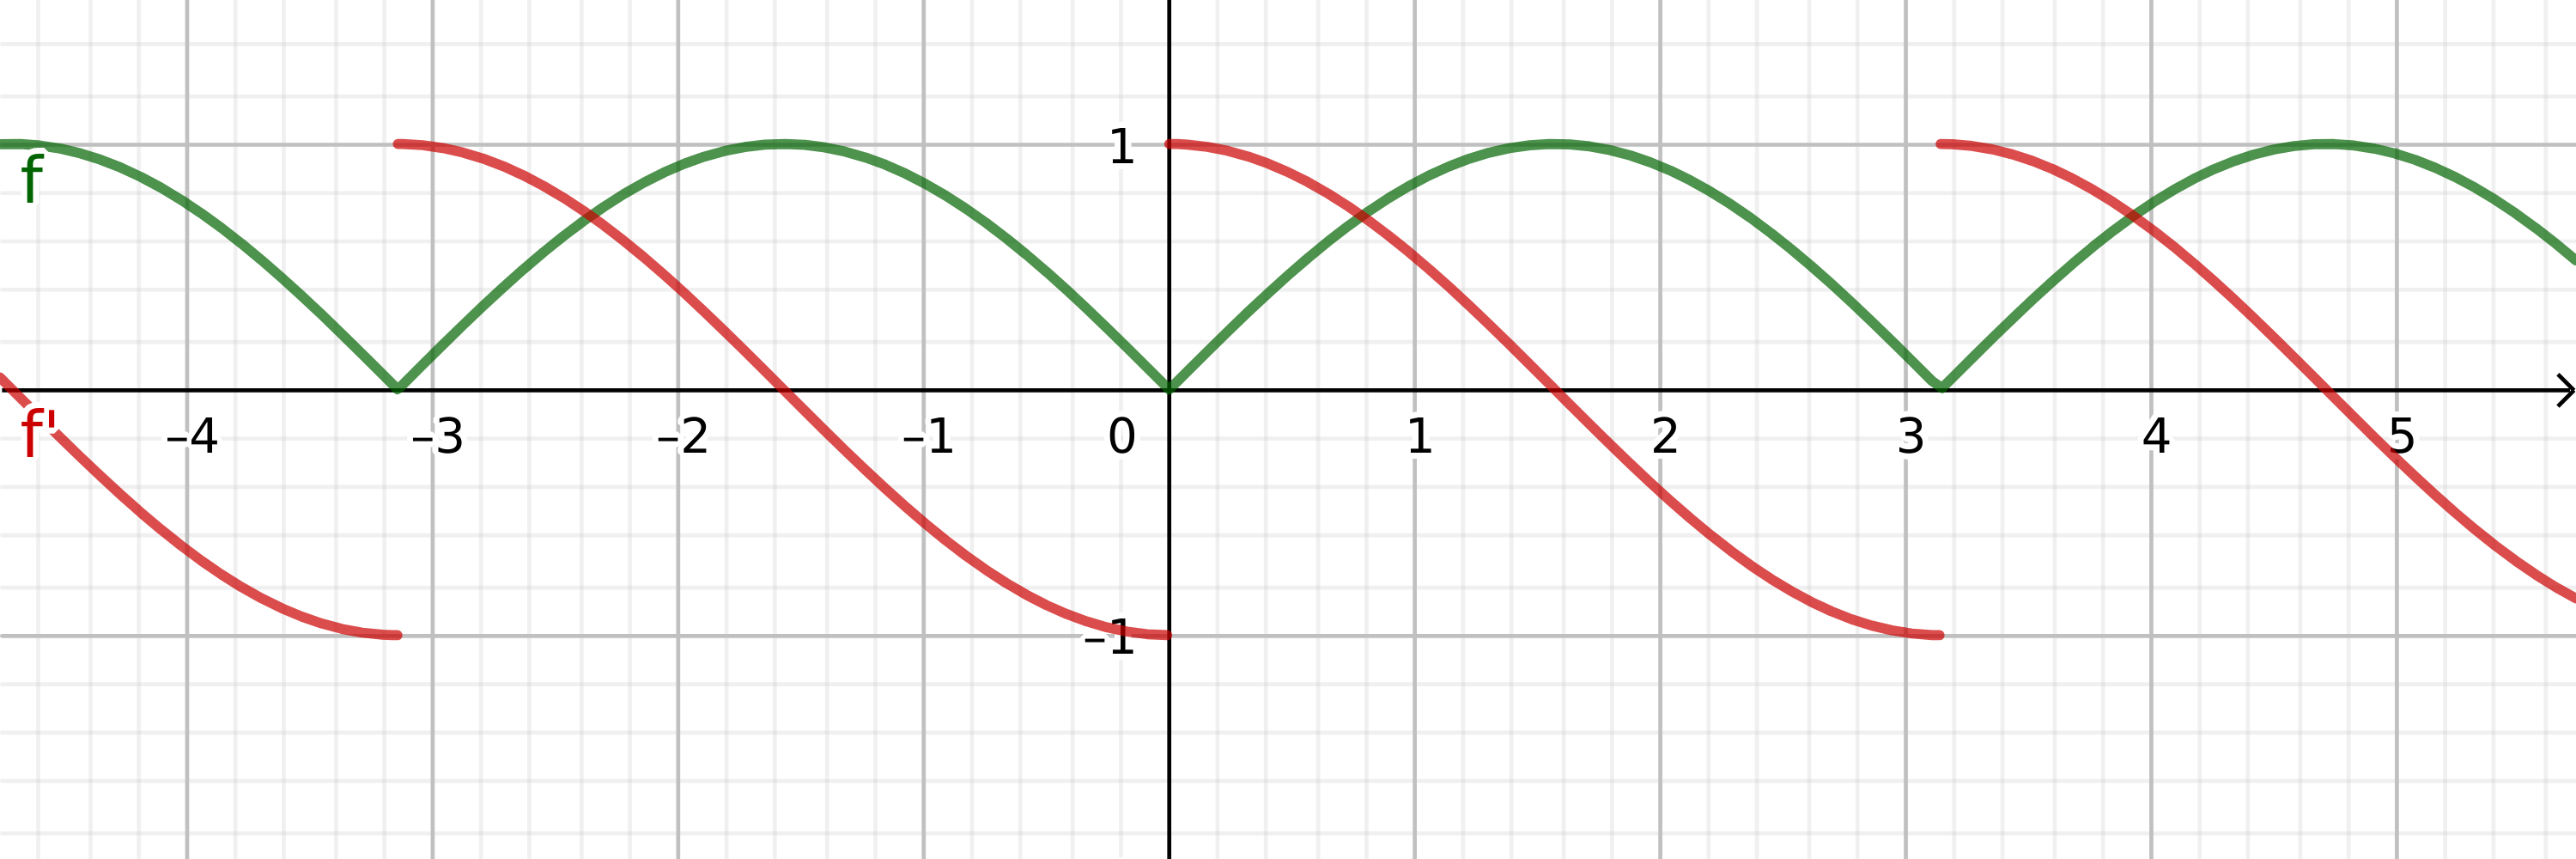
\includegraphics{96b.png}

    The green line represents $f(x)$, and the red line represents $f'(x)$.

    $f$ is not differentable at $x = k\pi$, where $k \in Z$.
    
    \subsection*{96. (c)}

    By the conclusion of problem (a), we can get $$g'(x) = \cos|x| (|x|)' = \cos|x| \frac{x}{|x|}$$
    
    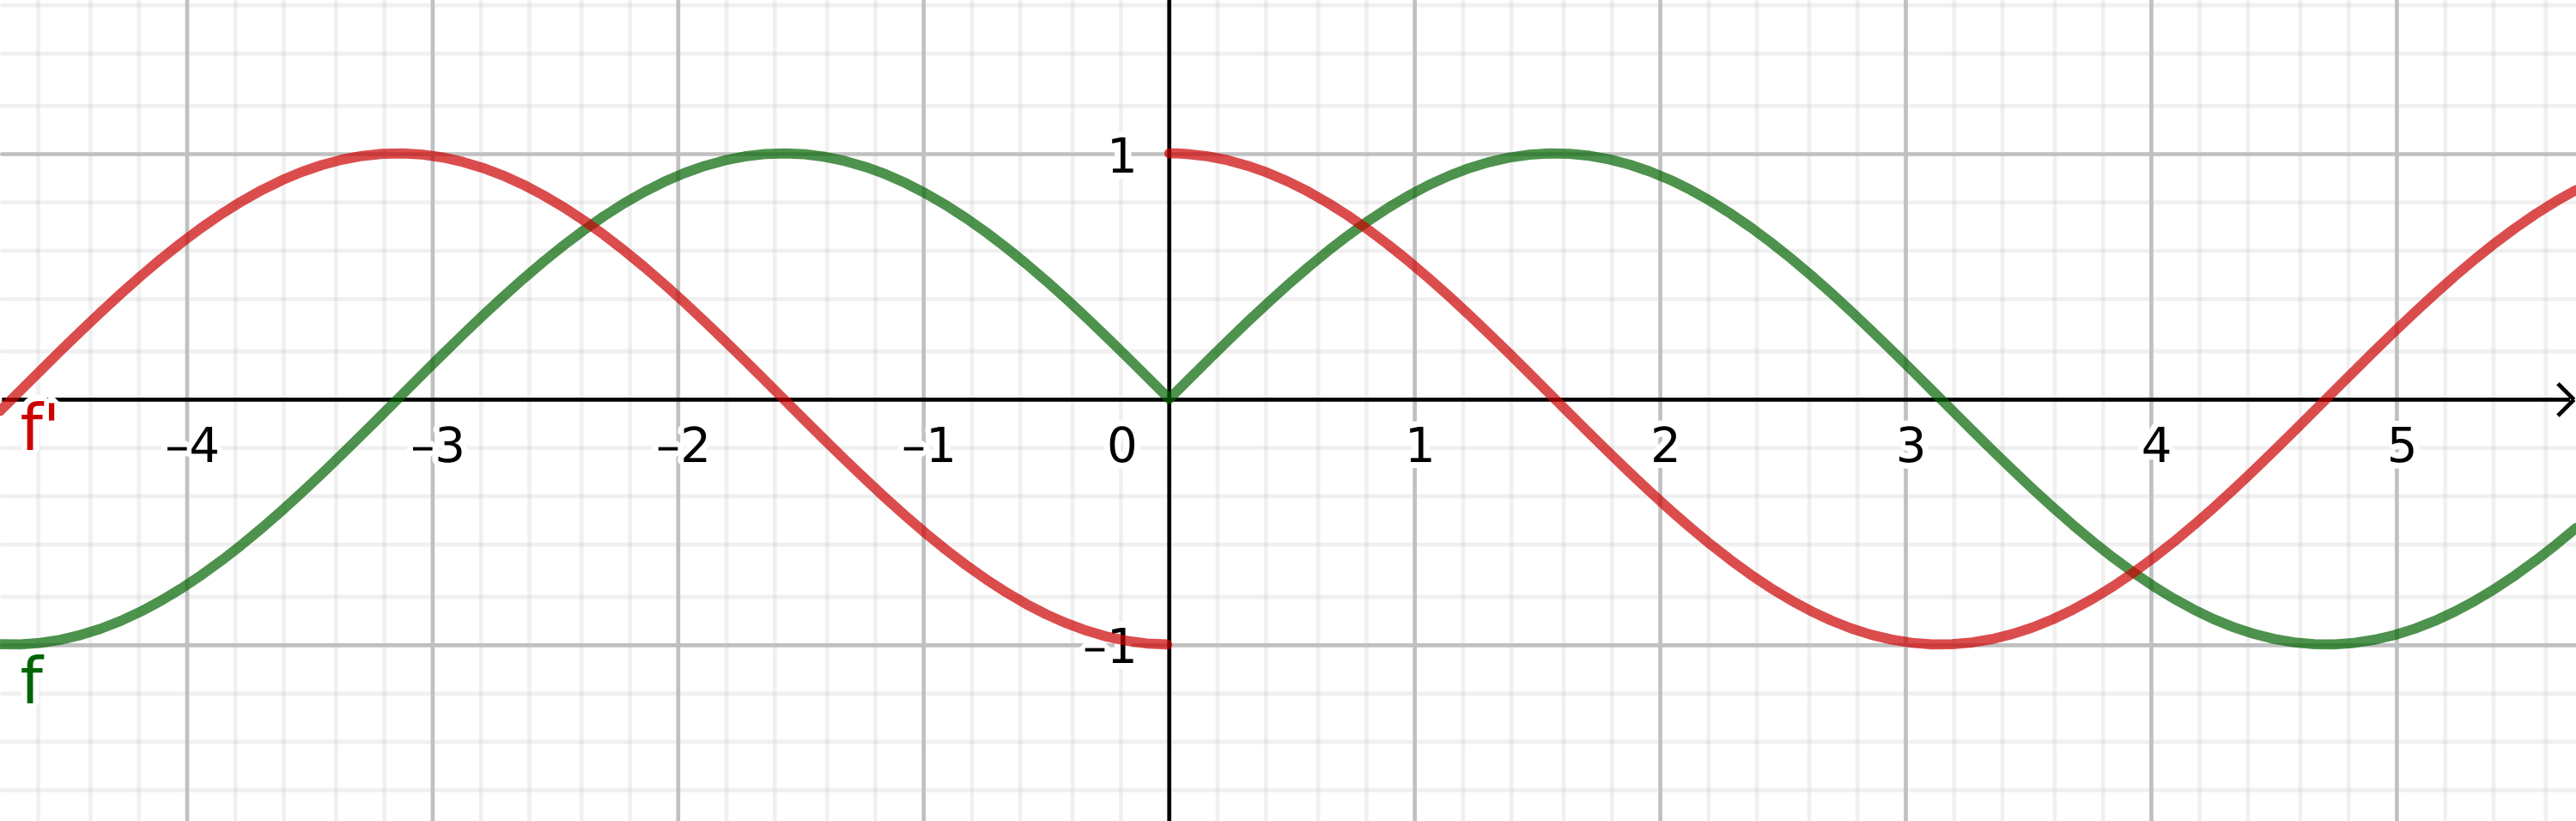
\includegraphics{96c.png}

    The green line represents $g(x)$ and the red line represents $g'(x)$.

    $g$ is not differentable at $x = 0$.

    \subsection*{97. If $y = f(u)$ and $u = g(x)$, where $f$ and $g$ are twice differentable functions, show that $$\frac{\mathrm d^2y}{\mathrm dx^2} = \frac{\mathrm d^2y}{\mathrm du^2}(\frac{\mathrm du}{\mathrm dx})^2 + \frac{\mathrm dy}{\mathrm du} \frac{\mathrm d^2u}{\mathrm dx^2}$$}
    
    $\because u = g(x), f'(u) = f'(u) g'(x)$

    $$\therefore f''(x) = [f'(u)]' = f''(u)g'(x) + f'(u)g''(x) = f''(u)u' + f'(u)u''$$

    $\therefore$ rewrite the formula in Leibniz's form, and we get
    $$\frac{\mathrm d^2y}{\mathrm dx^2} = \frac{\mathrm d^2y}{\mathrm du^2}(\frac{\mathrm du}{\mathrm dx})^2 + \frac{\mathrm dy}{\mathrm du} \frac{\mathrm d^2u}{\mathrm dx^2}$$

    \subsection*{98. If $y = f(u)$ and $u = g(x)$, where $f$ and $g$ possess third derivatives, find a formula for $\mathrm d^3y / \mathrm dx^3$ similar to the one given in Exercise 97.}

    By the conclusion of Exercise 97, we know $$f''(x) = [f'(u)]' = f''(u)g'(x) + f'(u)g''(x)$$

    $$\therefore f'''(x) = f'''(u)g'(x) + 2f''(u)g''(x) + f'(u)g'''(x)$$

    $\therefore$ rewrite the formula in Leibniz's form, and we get
    $$\frac{\mathrm d^3y}{\mathrm dx^3} = \frac{\mathrm d^3y}{\mathrm du^3} \frac{\mathrm du}{\mathrm dx} + 2 \frac{\mathrm d^2y}{\mathrm du^2}\frac{\mathrm d^2u}{\mathrm dx^2} + \frac{\mathrm dy}{\mathrm du} \frac{\mathrm d^3u}{\mathrm dx^3}$$


\end{document}
% 28 29 42 46 49 91 92 95 96 97 98